% \PassOptionsToPackage{usenames, dvipsnames}{color}
% \UseRawInputEncoding

\documentclass[12pt,usenames]{article}
\usepackage[a4paper, hmargin={2.8cm, 4.8cm}, vmargin={2.5cm, 2.5cm}, marginparwidth=100pt]{geometry}  % Geometri-pakke: Styrer bl.a. maginer    %
%%%%%%%%%%%%%%%%%%%%%%%%%%%%%%%%%%%%%%%%%%%%%%%%%%%%%%%%%%%%%%%%%%%%%%%%%
\usepackage[utf8]{inputenc}

\usepackage{algpseudocode}
\usepackage{algorithm}

\usepackage{amsthm}
\usepackage{amsfonts}
\newcommand{\Perp}{\perp \! \! \! \perp}
\usepackage{bm}
% \usepackage{txfonts}
\newcommand{\B}[1]{\mathbf{#1}}
\usepackage{mathtools}

\usepackage{float}

\usepackage{appendix}

\usepackage{graphicx}
\usepackage{caption}
\usepackage{subcaption}

\usepackage{xcolor}
\usepackage{minted}
\newtheorem{theorem}{Theorem}
\newtheorem{lemma}{Lemma}
\usepackage{listings}
\newcommand{\todo}[1]{\marginpar{\color{red}TODO:\color{black}\ #1}}
\newcommand{\const}{\textrm{const}}

\title{Bayesian Optimal Design - Weekly Report}
\author{Rasmus Hag Løvstad, \texttt{pgq596}}
\date{\today}

\graphicspath{ {./assets} }
\begin{document}
\maketitle
% \section{Week 1}
\subsection{Objective}
For week 1, we're going to explore the linear regression problem from a Bayesian perspective. 
First we are going to state essential model assumptions, from which we can examine the consequences of these using Bayes' rule.
This will be used to see how we can incorporate previous knowledge into the model and see how observing new data will change our model.
While this is apparent for any regression model, we will also demonstrate how we can actually derive an exact posterior parameter distribution in the case of linear regression.\\
In the end, we are going to implement a simple linear regression model in Python, and explore how the prior model assumptions affect our resulting model.
% The objective of this week is to explore the basics of probabilistic machine learning by implementing a Bayesian linear regression model 
% and explore how it is affected by its different hyperparameters like choice of prior as well as the variance and quantity of data points.
% \todo{Notes from meeting: Make 2D plot over parameter space that shows how the posterior moves from the prior. Update from Oswin's notes}
\subsection{Theory}
\subsubsection{The regression problem and Bayes' rule}
First, we are going to state the regression problem in general: 
Given a dataset $\mathcal{D} = (\B{d}, \B{y})$, where $\B{d}\in \mathbb{R}^{\ell \times d}$ and $\B{y} \in \mathbb{R}^{\ell}$, 
we wish to find some function $\phi_\theta \in \mathbb{R}^{\ell \times d} \rightarrow \mathbb{R}^{\ell}$ such that
\begin{equation}
  \label{eq:general-regression}
\phi(\B{d}) \approx \B{y}
\end{equation}
where $\phi$ takes some vector of parameters $\theta$.\\
In the Bayesian approach, we are going to describe the probability distribution of $\B{y}$ with no additional information as $p(\B{y})$, called the \textit{marginal}.
If we have observed any data $\B{d}$ and have some set of parameters $\theta$ such that equation \ref{eq:general-regression} is upheld, then we have additional information about the distribution of $\B{y}$.
This will be described as the \textit{likelihood} $p(\B{y} | \B{d}, \B{\theta})$.\\
We might have some prior information on how the parameters $\B{\theta}$ are distributed - perhaps from prior experiments, domain knowledge or qualified guessing. This can be encoded into the \textit{prior} distribution $p(\B{\theta})$.
Given a likelihood, a marginal, and a prior, we can use Bayes' rule to find the \textit{posterior} distribution of $\B{\theta}$ given the data $\B{d}$ and target values $\B{y}$:
\begin{equation}
  \label{eq:bayes-rule}
  p(\B{\theta} | \B{d}, \B{y}) = \frac{p(\B{y} | \B{d}, \B{\theta})p(\B{\theta})}{p(\B{y| \B{d}})}
\end{equation}
What the posterior distribution $p(\B{\theta} | \B{d}, \B{y})$ models is the \textit{change of belief} from the prior model $p(\theta)$ given the \textit{evidence} $p(\B{y} | \B{d})$, $\B{d}$\cite{krause22}.
It gives us a new best bet for the parameters $\B{\theta}$, which we can use to produce a better $\phi$ for equation $\ref{eq:general-regression}$.
%we wish to find a set of model parameters $\theta \in \mathbb{R}^{\ell \times d}$ such that 
\subsubsection{The linear regression problem}
In the case of linear regression, we assume that $\phi$ is a linear function, i.e. $\phi(\B{d}) = \B{d}\B{\theta}$ where $\B{\theta}\in \mathbb{R}^{d}$. 
It is also common to augment the dataset with an additional dimension set to 1, such that $\phi$ also models the intercept such that $\B{d} \in \mathbb{R}^{\ell \times d + 1}$ and $\theta \in \mathbb{R}^{d + 1}$. In this case $\theta_{d+1}$ will then be the intercept.\\

We are going to assume that the each target value $\B{y}$ can accurately be described as
\begin{equation}
  \label{eq:likelihood-generating}
  \B{y}^{(i)} = \B{d}^{(i)}\theta + \epsilon
\end{equation}
for some $\B{d}$, $\theta$, $\epsilon$, where $\epsilon \sim \mathcal{N}(0, \sigma^2_{\B{y}})$ is some normally distributed noise term.
Thus, the likelihood distribution can be described like a normal distribution.
\begin{equation}
  \label{eq:likelihood-single}
  p(\textbf{y}^{(i)} | \B{d}^{(i)}, \B{\theta}) = \mathcal{N}(\B{y}^{(i)}; \B{d}^{(i)}\B{\theta}, \sigma^2_{\B{y}})
\end{equation}
Assuming that the target values are independent, it must follow that
\begin{equation}
  \label{eq:likelihood}
  p(\textbf{y} | \B{d}, \B{\theta}) = \prod_{i=0}^\ell p(\textbf{y}^{(i)} | \B{d}^{(i)}, \B{\theta}) = \mathcal{N}(\B{y}; \B{d}\B{\theta}, \sigma^2_{\B{y}}I_\ell)
\end{equation}
When modelling the prior information, one could choose to model the parameter distribution as a multivariate gaussian distribution as well
\begin{equation}
  \label{eq:prior}
  p(\B{\theta}) = \mathcal{N}(\theta; \mu_{\theta}, \Sigma_\theta)
\end{equation}
where $\mu_\theta$, $\Sigma_\theta$ are chosen by the model designer.\\
The last term of equation \ref{eq:bayes-rule} is the marginal distribution $p(\B{y})$, which is the probability of observing the target values $\B{y}$ without any additional information. 
This term is difficult to make any reasonable assumptions about, and can thus hard to compute in practice.
Lukily, it mostly acts as a normalization term that makes sure that the posterior distribution integrates to 1, so it can for many use cases be safely ignored.
As we will see, for a linear regression problems with these assumptions, we will indeed not need it.
\subsubsection{An analytical solution for the posterior distribution}
Let us outline a possible derivation for the posterior distribution: Given the likelihood and prior, we can describe the joint distribution $p(\theta, \B{y} | \B{d})$ as
\begin{equation}
  \label{eq:joint}
  p(\theta, \B{y} | \B{d}) = p(\B{y} | \B{d}, \theta)p(\theta | \B{d}) = p(\B{y} | \B{d}, \theta)p(\theta)
\end{equation}
where the last equality is due to the model parameters being independent from the controlled data points. \\
From this point, we will need to condition the joint distribution on $\B{y}$:
\begin{equation}
  \label{eq:joint-conditioned}
  p(\theta | \B{y}, \B{d}) = \frac{p(\theta, \B{y} | \B{d})}{p(\B{y})}
\end{equation}
To perform these steps, we are going to use some useful lemmas about the multivariate normal distribution.
\begin{lemma}
  \label{lemma:block-conditional}
  Let $\B{X} \sim \mathcal{N}(\B{\mu}, \Sigma)$ be a multivariate normal random variable. We can regard these variables in block notation:
  \begin{equation}
  \B{X}=\begin{bmatrix}[c]
    \B{X}_1\\
    \hline
    \B{X}_2
  \end{bmatrix}, \quad \mu = \begin{bmatrix}[c]
    \mu_{1}\\
    \hline
    \mu_{2}
  \end{bmatrix},\quad \Sigma=\begin{bmatrix}[c|c]
  \Sigma_{11} & \Sigma_{12}\\
    \hline
    \Sigma_{21} & \Sigma_{22}
  \end{bmatrix}
\end{equation}
  then we must have
  \begin{equation}\mu_{2|1}=\mu_2 + \Sigma_{21}\Sigma_{11}^{-1}(X_1 - \mu_1),\quad \Sigma_{2|1} = \Sigma_{22} - \Sigma_{21}\Sigma_{11}^{-1}\Sigma_{21}^T\end{equation}
\end{lemma}
\begin{proof}
  See \citet{krause22} \todo{implement proof}
\end{proof}
\begin{lemma}
  \label{lemma:block-joint}
  For random variables $\B{X} \sim \mathcal{N}(\B{\mu}_\B{X}, \Sigma_\B{X})$, $\B{Y}|\B{X} \sim \mathcal{N}(\B{\mu}_\B{Y} + A\B{X}, \Sigma_\B{Y})$,
  for some $A$, the joint distribution $p(\B{X}, \B{Y})$ is given by
  \begin{equation}
    \begin{bmatrix}[c]
      \B{X} \\
      \hline
      \B{Y}
    \end{bmatrix}
    =
    \mathcal{N}\left(
      \begin{bmatrix}[c]
        \B{\mu}_\B{X} \\
        \hline
        \B{\mu}_\B{Y} + A\B{\mu}_\B{X}
      \end{bmatrix},
      \begin{bmatrix}[c | c]
        \Sigma_\B{X} & \Sigma_\B{X}A^T \\
        \hline
        A\Sigma_\B{X} & A\Sigma_\B{X}A^T + \Sigma_\B{Y}
      \end{bmatrix}
    \right)
  \end{equation}
\end{lemma}
\begin{proof}
  Follows from Lemma \ref{lemma:block-conditional} and the definition of the multivariate normal distribution.
\end{proof}
If we regard the likelihood from equation \ref{eq:likelihood}, we can see that it is only dependent of $\theta$ in its mean-term.
Thus we can use Lemma \ref{lemma:block-joint} to get the joint distribution $p(\theta, \B{y} | \B{d})$:
\begin{equation}
  \begin{bmatrix}[c]
    \theta \\
    \hline
    \B{y}
  \end{bmatrix}
  =
  \mathcal{N}\left(
    \begin{bmatrix}[c]
      \mu_\theta \\
      \hline
      \B{d}\mu_\theta
    \end{bmatrix},
    \begin{bmatrix}[c | c]
      \Sigma_\B{\theta} & \Sigma_\B{\theta}\B{d}^T \\
      \hline
      \B{d}\Sigma_\B{\theta} & \B{d}\Sigma_\B{\theta}\B{d}^T + \sigma^2_\B{y} I_\ell
    \end{bmatrix}
  \right)
\end{equation}
To get the posterior distribution, we will need to use the conditioning Lemma \ref{lemma:block-conditional} on a reordered term:
\begin{equation}
  \begin{bmatrix}[c]
    \B{y}\\
    \hline
    \theta 
  \end{bmatrix}
  =
  \mathcal{N}\left(
    \begin{bmatrix}[c]
      \B{d}\mu_\theta\\
      \hline
      \mu_\theta
    \end{bmatrix},
    \begin{bmatrix}[c | c]
      \B{d}\Sigma_\B{\theta}\B{d}^T + \sigma^2_\B{y} I_\ell &     \B{d}\Sigma_\B{\theta} \\ 
      \hline
      \Sigma_\B{\theta}\B{d}^T & \Sigma_\B{\theta}
    \end{bmatrix}
  \right)
\end{equation} \todo{remove d theta}
With the conditioning lemma, we get the posterior distribution $p(\theta | \B{y}, \B{d}) = \mathcal{N}(\theta; \mu_{\theta| \B{y}, \B{d}}, \Sigma_{\theta | \B{y}, \B{d}})$:
\begin{equation}
  \label{eq:posterior-mean}
  \mu_{\theta | \B{y}, \B{d}} = \mu_\theta + \Sigma_\theta \B{d}^T (\B{d} \Sigma_\theta \B{d}^T + \sigma^2_\B{y} I_\ell)^{-1}(\B{y} - \B{d}\mu_\theta)
\end{equation}
\begin{equation}
  \label{eq:posterior-cov}
  \Sigma_{\theta | \B{y}, \B{d}} = \Sigma_\theta - \Sigma_\theta \B{d}^T (\B{d} \Sigma_\theta \B{d}^T + \sigma^2_\B{y} I_\ell)^{-1}\B{d}\Sigma_\theta
\end{equation}
Thus we have an analytical expression for the posterior distribution.
\subsubsection{Using the posterior to optain model parameters}
From this distribution, we can optain model parameters in several ways. 
A common choice is to pick the $\theta$ that maximizes the posterior. This is called the \textit{Maximum-a-posteriori} (MAP) estimate, and will for a normal distribution just be the posterior mean $\mu_{\theta | \B{y}, \B{d}}$.
For other cases than linear regression, one can also use a mean over samples of $\theta$ from the posterior distribution, but for our case, this will converge against the posterior mean $\mu_{\theta | \B{y}, \B{d}}$.
Another solution is to define a distribution called the \textit{posterior predictive} distribution, that for some new data points $\B{d}_{\textrm{new}}$ computes the corresponding $\B{y}_{\textrm{new}}$:
\begin{equation}p(\B{y}_{\textrm{new}} | \B{d}_{\textrm{new}}, \B{d}, \B{y}) = \int p(\theta | \B{y}, \B{d}) p(\B{y}_{\textrm{new}} | \theta, \B{d}_\textrm{new})d\theta\end{equation}
Integrals like these are usually solved by sampling - examples of this will be seen later. For now, we can use Lemma \ref{lemma:block-joint} to get
\begin{equation}p(\B{y}_{\textrm{new}} | \B{d}_{\textrm{new}}, \B{d}, \B{y}) = \mathcal{N}(\B{y}_\textrm{new}; \B{d}_\textrm{new}^T\mu_{\theta|\B{y}, \B{d}}, \sigma^2_\B{y} + \B{d}_\textrm{new}^T\Sigma_{\theta | \B{y}, \B{d}}\B{d}_\textrm{new})\end{equation}
Having the posterior predictive allows us to both sample a $\B{y}$ for a given $\B{d}$, choose the $\B{y}$ that maximises the distribution, and to give us some measure of the inherent uncertancy in the model \cite{krause22}.
\subsubsection{Linear regression being invariant to translation}
A relevant side-note worth exploring is the effect of the choice of prior mean $\mu_\theta$ on the posterior mean $\mu_{\theta | \B{y}, \B{d}}$.

\todo{Finish this section with information from Oswin - and edit posterior predictive if needed}

\subsection{Implementation}
Implementing a Bayesian linear regression model is fairly simple.
To begin with, one needs to decide on a prior distribution for $\theta$, as well as what the variance of the noise $\sigma^2_\B{y}$ should be used to generate the example data.
In the real world, $\sigma^2_\B{y}$ would be measured from observed data, and the prior would be chosen based on the expected distribution of $\theta$ based on as much prior knowledge as possible
, but for our toy representation, we are going to play around with many different possible priors and noise parameters.
For a toy implementation, one can start by generating some data points $\B{d}$ and noise samples $\epsilon$ as well as deciding on some true, underlying weight parameters $\theta_{\textrm{true}}$.
Then we can compute $\B{y}$ as in equation \ref{eq:likelihood-generating}. 
From this, we can simply implement the posterior distribution as in equation \ref{eq:posterior-mean} and \ref{eq:posterior-cov}.
In Python, this can be done as follows:
\begin{minted}{python}
def posterior_distribution(theta, d, y):
    mu = cov_prior @ d.T @ np.linalg.inv(d @ cov_prior @ d.T + noise * np.eye(l)) @ y
    cov = cov_prior - cov_prior @ d.T @ np.linalg.inv(d @ cov_prior @ d.T + noise * np.eye(l)) @ d @ cov_prior
    return stats.multivariate_normal.pdf(theta, mean=mu, cov=cov)
\end{minted}

\subsection{Results}
An example of how 20 samples of $\theta$ from the posterior changes with the size of the dataset can be seen in Figure \ref{fig:fixed-prior}.
As one can see, the posterior becomes better at estimating the true $\theta$ as the number of data points increases,
since the lines both become more similar and closer to the mean, as well as how they describe the data better. \\
An example of how the posterior changes from the prior can be seen in figure \ref{fig:random-prior}, where 40 random prior means and covariances are plotted alongside their respective posterior.
It can be seen that even when the priors are very different, the posterior usually ends up quite close to the true weight.
An example of how the posterior predictive distribution changes is seen in figure \ref{fig:posterior-predictive}.
As one can see, the distribution becomes less confident as the noise increases. \\
Thus we've seen that the Bayesian linear regression model is able to learn the true weight parameters from data, and that it is able to do so even when the prior is very different from the true weight parameters. Now, we will move on to regarding the Bayesian Optimal Design problem.
\todo{Make plots nicer, add "true" line for reference, add legend}
\begin{figure}[H]
\begin{subfigure}{.5\textwidth}
  \centering
  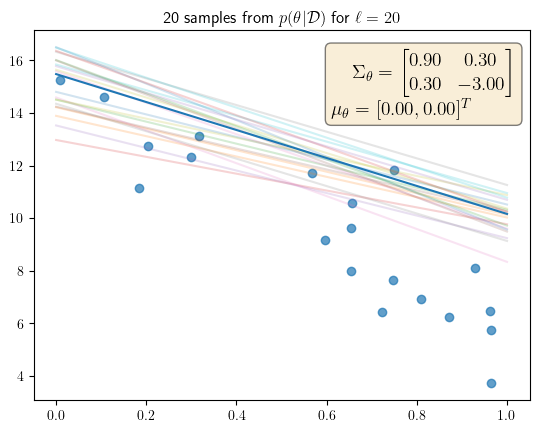
\includegraphics[width=0.8\textwidth]{assets/week1/fixed-prior-20-samples.png}
\end{subfigure}%
\begin{subfigure}{.5\textwidth}
  \centering
  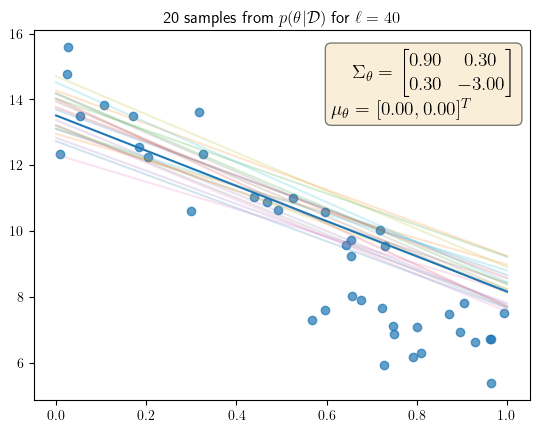
\includegraphics[width=0.8\textwidth]{assets/week1/fixed-prior-40-samples.png}
\end{subfigure}\\
\begin{subfigure}{1\textwidth}
  \centering
  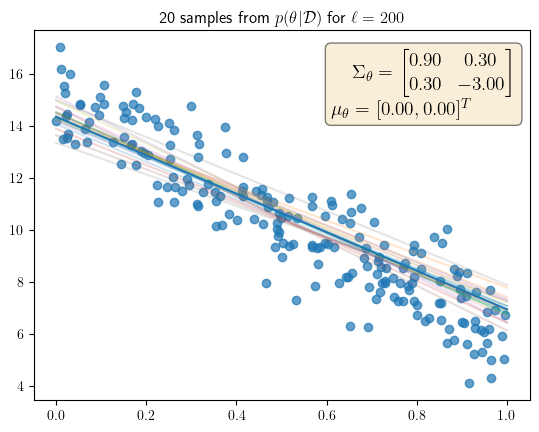
\includegraphics[width=0.4\textwidth]{assets/week1/fixed-prior-200-samples.png}
\end{subfigure}%
\caption{The model trained on data sets with 20, 40 and 200 data points respectively with a fixed prior. The blue line is $\mu_{\theta|\mathcal{D}}$.}
\label{fig:fixed-prior}
\end{figure}

\begin{figure}[H]
\begin{subfigure}{1\textwidth}
  \centering
  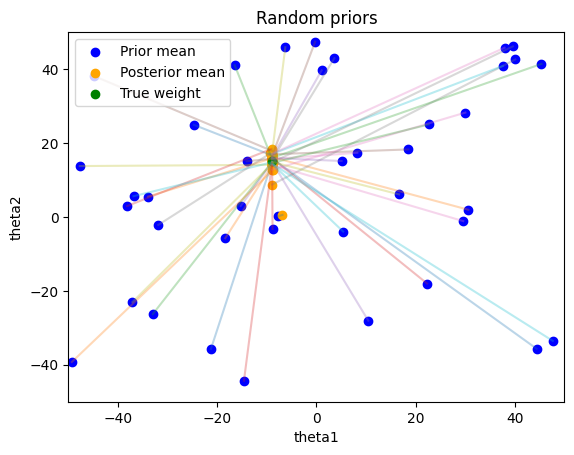
\includegraphics[width=0.7\textwidth]{assets/week1/random-priors.png}
  \caption{Plot showing how the posterior mean changes compared to the prior mean.}
\end{subfigure}\\
\begin{subfigure}{.5\textwidth}
  \centering
  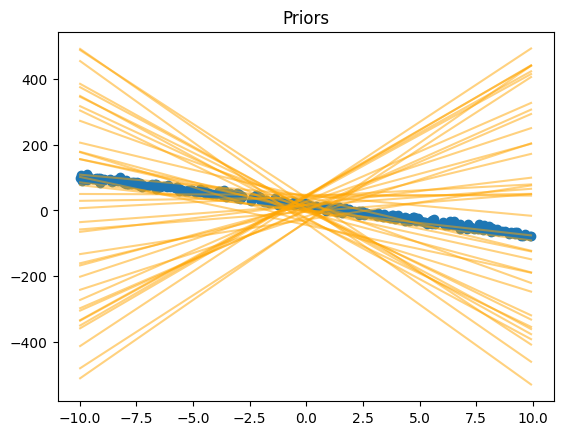
\includegraphics[width=0.8\textwidth]{assets/week1/random-priors-plot.png}
  \caption{Prior mean samples}
\end{subfigure}%
\begin{subfigure}{.5\textwidth}
  \centering
  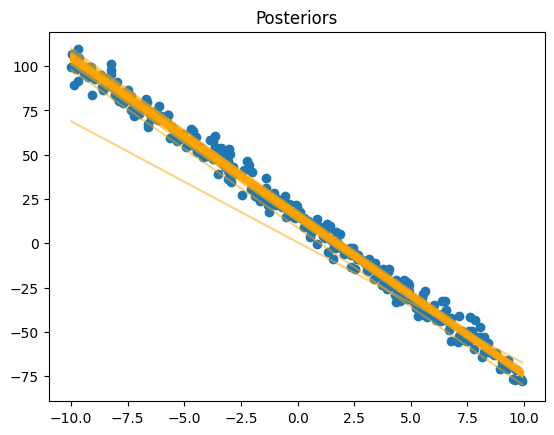
\includegraphics[width=0.8\textwidth]{assets/week1/random-priors-posteriors.png}
  \caption{Posterior mean samples}
\end{subfigure}
\caption{Priors vs Posteriors for 40 randomly sampled priors on the same data set. Note that the variance is due to random prior covariances.}
\label{fig:random-prior}
\end{figure}

\begin{figure}[H]
\begin{subfigure}{1\textwidth}
  \centering
  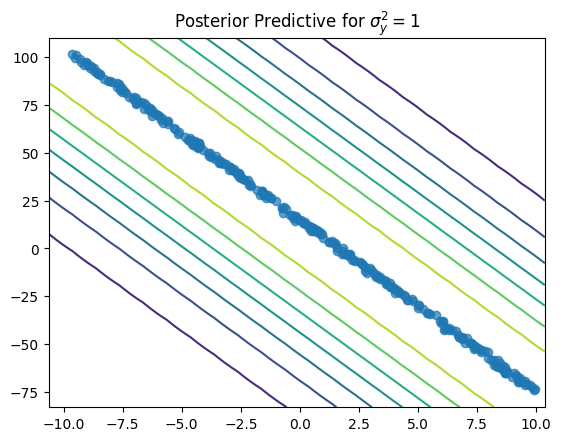
\includegraphics[width=0.5\textwidth]{assets/week1/noise-1.png}
\end{subfigure}\\
\begin{subfigure}{.5\textwidth}
  \centering
  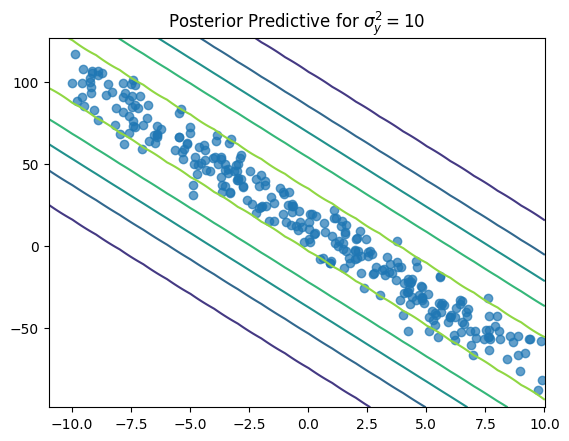
\includegraphics[width=0.8\textwidth]{assets/week1/noise-10.png}
\end{subfigure}%
\begin{subfigure}{.5\textwidth}
  \centering
  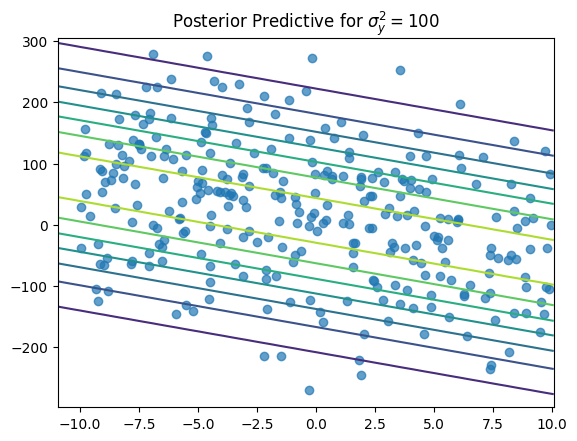
\includegraphics[width=0.8\textwidth]{assets/week1/noise-100.png}
\end{subfigure}
\caption{Posterior predictive for different noise levels}
\label{fig:posterior-predictive}
\end{figure}

% \section{Week 2}
\subsection{Objective}
For week 2, we are going to regard the \textit{Bayesian Optimal Design} problem for linear regression, and use this to implement a reference implementation, to be used later.
We can then also explore the effect of different data sizes, different priors and the difference between estimating an objective function through sampling versus calculating it analytically.
\subsection{Theory}
\subsubsection{Bayesian Optimal Design}
Often in scientific contexts as well as other cases, one might have a model that one wishes to strengthen in one way or another using experimental data.
Performing the experiments needed to strengthen one's model can be expensive however, so having an efficient strategy to do such can save important ressources.
This is where \textit{Bayesian Optimal Design} comes in.

The Bayesian Optimal Design problem is about finding a design $\B{d}$ from a design space $\B{D}$, that optimizes some kind of utility function.\cite{ryan15} 
For this project, we wish to maximize the expected information gain from the prior to the posterior.
% For this project, that utility function is the mutual information gained from an experiment by measuring at "location" $\B{d}$.\\
To find the optimal design, we want to find a maximizer $\B{d}^*$ defined as such:
\begin{equation}\label{eq:bayesian-optimal}\B{d}^* = \arg \max_{\B{d}\in \B{D}} I(\B{d})\end{equation}
Where $I(\B{d})$ is the \textit{Mutual Information} between the prior and posterior when adjusted for data observed at $\B{d}$.\\
\subsubsection{The Nature of the Mutual Information metric}
The amount of information of an experiment is often defined as the negative differential entropy defined as such\cite{lindley56}:
\begin{equation}H(X) = \int_{X}p(x)\log p(x)dx\end{equation}
Thus, the information known before $\B{y}$ is observed from $\B{d}$ is
\begin{equation}\label{eq:entropy-prior}H_1 = \int_{\Theta}p(\theta)\log p(\theta)d\theta\end{equation}
and after is
\begin{equation}\label{eq:entropy-posterior}H_2(\B{y}, \B{d}) = \int_{\Theta}p(\theta| \B{y}, \B{d})\log p(\theta| \B{y}, \B{d})d\theta\end{equation}
The gain of information must thus be
\begin{equation}H_\textrm{gain}(\B{y}, \B{d}) = H_2(\B{y}, \B{d}) - H_1\end{equation}
If we instead regard equation \ref{eq:entropy-prior} and \ref{eq:entropy-posterior} as expectations we get
\begin{equation} = \mathbb{E}_\theta[\log p(\theta | \B{y}, \B{d})] - \mathbb{E}_\theta [\log p(\theta )]  = \mathbb{E}_\theta [\log(p(\theta | \B{y}, \B{d})) - \log(p(\theta))]\end{equation}
Before we perform the experiment, we do not know what the outcome will be. Instead, we'll just regard the expected outcome by taking the expectation over $\B{y}$:
\begin{equation} \label{eq:mi}\mathbb{E}_\B{y}[H_\textrm{grain}(\B{y}, \B{d})]  = \mathbb{E}_\B{y}[\mathbb{E}_\theta [\log(p(\theta | \B{y}, \B{d})) - \log(p(\theta))]]\end{equation}
This expression is called the \textit{Mutual Information} between the prior and posterior, and will be denoted $I(\B{d})$.
We can put a new interpretation upon this by expanding equation \ref{eq:mi} using Bayes' rule:
\begin{equation} I(\B{d})  = \mathbb{E}_\B{y}[\mathbb{E}_\theta [\log(p(\B{y} | \B{\theta}, \B{d})) - \log(p(\B{y}|\B{d}))]]\end{equation}
Then we can use that $\frac{p(\B{y}, \B{\theta}|\B{d})}{p(\theta)}=p(\B{y| \theta, \B{d}})$:
\begin{equation} I(\B{d})  = \mathbb{E}_\B{y}[\mathbb{E}_\theta [\log\left(\frac{p(\B{y}, \B{\theta}|\B{d})}{p(\theta)}\right) - \log(p(\B{y}|\B{d}))]] = \mathbb{E}_\B{y}[\mathbb{E}_\theta [\log\left(\frac{p(\B{y}, \B{\theta}|\B{d})}{p(\theta)p(\B{y}|\B{d})}\right)]]\end{equation}
$$ = \textsc{KL}(p(\B{y}, \theta | \B{d})|| p(\theta)p(\B{y}|\B{d}))$$
Two random variables $X$ and $Y$ are said to be \textit{independent} if the product of their distributions is the same as their joint distribution i.e.
\begin{equation}p(X,Y) = p(X)p(Y)\end{equation}
Thus, Mutual Information measures how close the prior and the evidence \todo{check if indeed this is evidence}are to be independent. 
If $\B{d}$ is picked such that the prior has a high probability of being able to predict $\B{y}|\B{d}$, then the mutual information is going to be close to 0. 
If, on the contrary, $\B{d}$ is picked such that the prior has a low probability of being able to predict $\B{y}|\B{d}$, the mutual information is going to be large.
Thus one could expect that an optimizer would prefer to pick a $\B{d}$ within an area where the prior is not very representative of the underlying generating function.
Of course, in an experimental design context we do not have access to this underlying function as we might not be able to simulate experiments accurately. Instead, the expectation expressions in \ref{eq:mi}
makes it such that we only regard the expected information gain for any given underlying function.

\subsubsection{Evaluating the Mutual Information through sampling}
Without using any assumptions about the nature of our model or data, we can utilize Monte Carlo sampling to optain an accurate estimate on the expectations in equation \ref{eq:mi}.
For $N$ samples of $\theta \sim p(\theta)$ and $M$ samples of $\B{y} \sim p(\B{y} | \theta, \B{d})$ this thus looks like
\begin{equation}
  I(\B{d}) \approx \frac{1}{NM}\sum_{i=0}^N\sum_{j=0}^M(\log (p(\theta_i | \B{y}_j, \B{d})) - \log(p(\theta_i)))
\end{equation}
Picking samples of $\B{y}$ nescessitates that we can simulate the experiment however.
Instead, we will use the reparamerization trick to sample M samples of $\B{z}\in \mathcal{N}(0, 1)$ such that
\begin{equation}
  \B{y}_{ij} = \mu_{\B{y}| \theta, \B{d}} + A_{\B{y}| \theta, \B{d}}\B{z}_j
\end{equation}

where $A_\B{y}$ is a matrix such that $A_\B{y}A_\B{y}^T = \Sigma_\B{y}$. 
From equation \ref{eq:likelihood} we have that $p(\B{y}| \theta, \B{d}) = \mathcal{N}(\B{y}; \B{d}\theta, \sigma^2_\B{y}I_n)$ so we must have $A_{\B{y}|\theta, \B{d}} = \sigma^2_{\B{y}}I_n$
thus 
\begin{equation}
  \label{eq:mi-sampled}
  I(\B{d}) \approx \frac{1}{NM}\sum_{i=0}^N\sum_{j=0}^M(\log (p(\theta_i | \B{d} \theta_i + \sigma^2_{\B{y}}\B{z}_j, \B{d})) - \log(p(\theta_i)))
\end{equation}

\subsubsection{Evaluating the Mutual Information through analytical solutions}
It also happens that when we transform equation \ref{eq:mi} using sum of expectations, one can use the known solution to entropy of multivariate normal distributions:
\begin{equation} I[(\B{y}, \B{d})]  = \mathbb{E}_\B{y}[\mathbb{E}_\theta [\log(p(\theta | \B{y}, \B{d}))]] - \mathbb{E}_\theta[\log(p(\theta))]\end{equation}
$$= \mathbb{E}_{\B{y}}[\frac{1}{2}\ln \det (2\pi e \Sigma_{\theta|\B{y,d}})] - \frac{1}{2}\ln \det (2\pi e\Sigma_\theta)$$
It also happens to be that $\Sigma_{\theta|\B{y,d}}$ is independent from $\B{y}$, as we saw last week, thus we get.
\begin{equation} I[\B{y}, \B{d}]  = \frac{1}{2}\ln \det (2\pi e \Sigma_{\theta|\B{y,d}}) - \frac{1}{2}\ln \det (2\pi e\Sigma_\theta)\end{equation}

\subsubsection{Stochastic Optimization}
For the sampling approach here, and in the rest of the project, we will use a stochastic gradient descent algorithm to perform the optimization nescessary to solve \ref{eq:bayesian-optimal}.
From some starting point $\B{d}_0$, iteratively update $\B{d}_i$ by
\begin{equation}
  \B{d}_i = \B{d}_{i-1} + \alpha \frac{1}{10^c + i \times 10^{-\beta}} \nabla_{\B{d}} I(\B{d}_{i-1})
\end{equation}
where $\alpha, \beta, c \in \mathbb{R}$ are hyperparameters that ensures a slow converges to taylor the natural variance that occurs when using Monte Carlo methods.

\subsection{Implementation}
The mutual information metric can be implemented using the sampling method like so:
\begin{minted}{python}
def mutual_information(d):
  N = 50 # amount of theta samples
  M = 50 # amount of z samples
  thetas = np.random.multivariate_normal(mean_prior, cov_prior, N)
  zs = np.random.randn(M)
  results = []
  for theta in thetas:
    ys = np.array([d @ theta + sigma_y * z for theta in thetas for z in zs])
    for y in ys:
      log_posterior = np.log(posterior_distribution(theta, d, y)) # using posterior_distribution from last week
      log_prior = multivariate_normal.logpdf(theta, mean_prior, cov_prior)
      results.append(log_posterior - log_prior)
  return np.mean(results)
\end{minted}

And using the analytical solution like so:
\begin{minted}{python}
def mutual_information(d):
  cov_posterior = get_cov_posterior(d) # using method from from last week
  return 0.5 * np.log(np.linalg.det(2*np.pi*np.e*cov_posterior)) - 0.5 * np.log(np.linalg.det(2*np.pi*np.e*covariance_prior))
\end{minted}

Finding the gradient of these solutions can be done using \texttt{autograd.grad}. 
An example of this can be seen in this implementation of the gradient descent algorithm:
\begin{minted}{python}
def optimize(f, d0, alpha, beta, c, iterations):
  d = d0
  g = grad(f)
  for i in range(iterations):
    d = d + alpha / (10**c + i * 10**(-beta)) * g(d)
  return d
\end{minted}

\subsection{Results}
If we regard the problem with $\ell = 10$ datapoints and $d=2$ dimensions with a zero-prior mean and identity prior covariance, 
we will data that is closer to the optimum to be spread out wider and more evenly in the parameter space.
This can be seen if one regards equation \ref{eq:mi-sampled}. 
If $\B{d}$ is picked such that $\B{d}\theta_i$ has a high probability of being a small number, then
$\B{d}\theta_i + \sigma^2_\B{y}\B{z}_j$ is going to get dominated by the noise term $\sigma^2_\B{y}\B{z}_j$.
Thus, the log-posterior $\log p(\theta_i | \B{d}\thta_i + \sigma^2_\B{y}\B{z}_j, \B{d})$ will be smaller.
If on the other hand, $\B{d}$ is picked such that $\B{d}\theta_i$ has a high probability of being a large number, then $\B{d}\theta_i$ is going to dominate the noise term
and the posterior has a higher probability of being a large number.\\
In figure \ref{fig:mi-2d}, we can see if start position of 11 datapoints are on top of eachother, all at $(0;0)$, they will swiftly move to a more spread out formation.
\begin{figure}
  \centering
  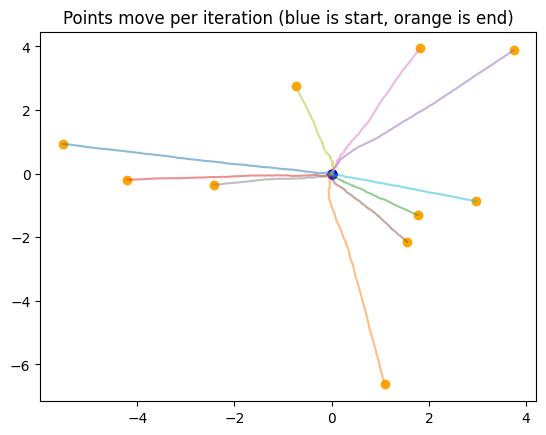
\includegraphics[width=0.8\textwidth]{week2/mi-2d.png}
  \caption{Points moving from their initial position at (0;0) to a more optimal, spread out position.}
  \label{fig:mi-2d}
\end{figure}
Thus we've seen how optimizing over the Mutual Information metric can help find solutions to the Bayesian Optimal Design problem.
Now we will move on to exploring how to solve regression problems, even when analytical solutions are not available with the hopes of opening up our Mutual Information optimizer to all kinds of models.

\section{Week 3-4}
\subsection{Objective}
This week, we will study and implement the variational inference framework with the objective of
estimating the posterior in a way that is indifferent to the type of regression performed.
We are going to pose the problem as an optimization problem and then derive an objective function that we can optimize over.
We will then try to implement it and perform some adjustments for efficiency and numerical stability.
% The objective of this week is to learn about and implement variational inference for Bayesian linear regression. 
% Then we will study convergence rates and accuracy by playing around with different parameters.
\subsection{Theory}
\subsubsection{Variational Inference and Variational Families}
In week 1, we were able to calculate the exact posterior using the right assumption and conjugacy between the prior and likelihood.
This turns out to be a rarity - in most cases, a closed form solution for the posterior is not readily available.
A common approach to this problem is to approximate the posterior distribution, using a \textit{variational distribution} $q$ picked from a family of distributions 
that we might imagine could approximate the posterior.
By picking a suitable objective function, we can use optimization techniques to pick a suitable $q$.
This is called \textit{variational inference}. Thus, our goal is to find a $q$ such that for any $\theta\in \Theta$, $q(\theta) \approx p(\theta | \B{y}, \B{d})$.
\subsubsection{Deriving a suitable objective function}
Without any further assumptions about our variational distribution, an immediate idea could be to use the KL-divergence between $q$ and $p$ as an objective function:
\begin{equation}\label{eq:kld}q^*(\theta) = \arg \min_{q} \textsc{KL}(q(\theta) || p(\theta | \B{y}, \B{d}))\end{equation}
Calculating this requires us to calculate the posterior, which we would like to avoid since we are often not guaranteed to be able to compute the evidence term $\log(p(\B{y} | \B{d}))$ from \eqref{eq:bayes-rule}.
We can however rewrite the KL-divergence as follows \cite{blei17}:
\begin{equation}\textsc{KL}(q(\theta)|| p(\theta| \B{y}, \B{d})) = \mathbb{E}_{\theta \sim q}[\log q(\theta)] - \mathbb{E}_{\theta \sim q}[\log p(\theta|\B{y}, \B{d})]\end{equation}
and by conditioning
\begin{equation}\label{eq:kld-2}= \mathbb{E}_{\theta \sim q}[\log q(\theta)] - \mathbb{E}_{\theta \sim q}[\log p(\theta, \B{y}| \B{d})] - \log p(\B{y}| \B{d})\end{equation}
One can now notice that the last term is actually constant with regards to $q$.
Thus, when we optimize, we can ignore it. The remaining terms form the negative \textit{evidence lower bound} (ELBO) \cite{blei17}:
\begin{equation}\label{eq:elbo-1}\textsc{ELBO}(q)= -\textsc{KL}(q(\theta) || p(\theta | \B{y}, \B{d})) + \textrm{const}= \mathbb{E}_{\theta \sim q}[\log p(\theta, \B{y}| \B{d})]-\mathbb{E}_{\theta \sim q}[\log q(\theta)]\end{equation}
Since the KL-divergence consists of the negative ELBO and a constant, we can minimize the KL-divergence by maximizing the ELBO. Thus, we can reformulate our objective:
\begin{equation}\label{eq:elbo-objective}q^*(\theta) = \arg \max_{q} \textsc{ELBO}(q)\end{equation}
We can derive \eqref{eq:elbo-1} to a more easily computable term:
\begin{equation}\label{eq:elbo-2}\textsc{ELBO}(q) = \mathbb{E}_{\theta \sim q}[\log (p(\B{y}| \theta , \B{d})p(\theta | \B{d}))] - \mathbb{E}_{\theta \sim q}[\log q(\theta)]\end{equation}
\begin{equation}= \mathbb{E}_{\theta \sim q}[\log p(\B{y}| \theta , \B{d})]+\mathbb{E}_{\theta \sim q}[\log p(\theta | \B{d})] - \mathbb{E}_{\theta \sim q}[\log q(\theta)]\end{equation}
Using that $\theta$ is independent of $\B{d}$, we have
\begin{equation}= \mathbb{E}_{\theta \sim q}[\log p(\B{y}| \theta , \B{d})]-(-\mathbb{E}_{\theta \sim q}[\log p(\theta)] + \mathbb{E}_{\theta \sim q}[\log q(\theta)])\end{equation}
\begin{equation}= \mathbb{E}_{\theta \sim q}[\log p(\B{y}| \theta , \B{d})]-\mathbb{E}_{\theta \sim q}\left[\log \left(\frac{q(\theta)}{p(\theta)}\right)\right]\end{equation}
Using the definition of the KL-divergence:
\begin{equation}\label{eq:elbo-3}= \mathbb{E}_{\theta \sim q}[\log p(\B{y}| \theta , \B{d})]- \textsc{KL}(q || p)\end{equation}
Thus, this variational inference problem can work for any posterior, as long as one can calculate the expectation of the likelihood, and the KL-divergence between the variational distribution and the prior.
\subsubsection{The Linear Regression Case}
Let us now look at how one can find a good variational family for the linear regression case.
An easy guess would be to pick $q$ from a family of multivariate Gaussian distributions, since we know from conjugacy between the prior and likelihood that the posterior must also be multivariate Gaussian.
Thus, one can expect $q^*$ to be able to estimate $p$ perfectly.\\
This has the nice consequence of turning the KL-divergence into a closed form expression, since both $q$ and $p$ follow multivariate normal distributions \cite{kld-gaussian}.\\
\begin{equation}\textsc{KL}(q || p) = \frac{1}{2}\left(\tr (\Sigma_p^{-1}\Sigma_q) + (\mu_p -\mu_q)^T\Sigma_p(\mu_p - \mu_q) - k + \log \frac{|\Sigma_p|}{|\Sigma_q|}\right)\end{equation}
We do have a problem, however: The first expectation of \eqref{eq:elbo-3} is an integral without a closed-form solution.
Thus, we wish to approximate it using Monte Carlo integration. 
To be able to sample $\theta$s from $q$, we will need to use the reparameterization trick:
By property of the multivariate normal distribution, there must exist some matrix $\B{A}$ such that $\theta \sim \mathcal{N}(\mu, \B{A} \B{A}^T)$ \cite{krause22}
and such that
\begin{equation}\theta = \mu + \B{A}\B{z}, \quad \textrm{where}\ \B{z}\sim \mathcal{N}(0,I_d)\end{equation}
Thus, we can simply sample N samples of $\B{z}$ and calculate $\theta$ from that. 
This means that our ELBO estimate can be written as follows:
\begin{equation}\textsc{ELBO}(q) \approx \frac{1}{N}\sum_{i=0}^N [\log p(\B{y} | \mu + \B{A}\B{z}^{(i)}, \B{d})] - \textsc{KL}(q || p)\label{eq:final-elbo}\end{equation}
$\mu$ and $\B{A}$ are then the parameters of $q$ that we will try to find through optimization.
% \subsubsection{Appendum: Using the ELBO as a proxy for the KL-divergence}
% When going from equation \ref{eq:kld-2} to \ref{eq:elbo-1}, we saw how the $\textsc{ELBO}$ is defined as the negative KLD plus the log-evidence $\log p(\B{y}|\B{d})$.
% The difference between the ELBO and the KLD is exactly this: the log-evidence.
\subsection{Implementation}
\subsubsection{Main implementation}
The main work of the algorithm is in calculating the ELBO. This can then be plugged into the same optimizer as in week 2.
The ELBO can be implemented as follows in Python:
\begin{minted}{python}
def ELBO(d, y, mean, A): # optimizing for mean, A
  zs = np.random.normal(size=(N, len(mean))) # N samples of size d
  likelihood_samples = []
  for z in zs:
    theta = mean + A @ z
    likelihood_samples.append(log_likelihood(y, theta, d))
  return 1/N * np.sum(likelihood_samples, axis=0) - KLD(mean, A, prior_mean, prior_A)
\end{minted}
where the log-likelihood is implemented after \eqref{eq:likelihood}:
\begin{minted}{python}
def log_likelihood(y, theta, d):
  return log_pdf(y, theta @ d, noise * np.eye(len(theta)))
\end{minted}
and the KL-divergence like so
\begin{minted}{python}
def KLD(mean_q, A_q, mean_p, A_p):
    sigma_q = (A_q @ A_q.T)
    sigma_p = (A_p @ A_p.T)
    bar_sigma_q = np.linalg.det(sigma_q)
    bar_sigma_p = np.linalg.det(sigma_p)
    k = len(mean_q)
    return 0.5 * (np.trace(np.linalg.inv(sigma_p) @ sigma_q) + (mean_p - mean_q).T @ np.linalg.inv(sigma_p) @ (mean_p - mean_q) - k + np.log(bar_sigma_p/bar_sigma_q))
\end{minted}
\subsubsection{Optimizing over a mean and a matrix}
Like in week 2, it is not trivial to optimize over both a mean and a matrix. Thus, we will encode $\mu$ and $\B{A}$ as a vector $\B{v}$ of the shape
$$\B{v}=\begin{bmatrix}\mu_0 \\ \vdots \\ \mu_d \\ \B{A}_{1,1} \\ \vdots \\ \B{A}_{1,d} \\ \B{A}_{2,1} \\ \vdots \\ \B{A}_{d, d}\end{bmatrix}$$
whenever we need to take the gradient or regard them in the context of the optimizer.
The following help functions can help encode and decode $\mu$ and $\B{A}$:
\begin{minted}{python}
def encode_q_params(q_params): # mean, A to vector
    mean, A = q_params
    return np.array(list(mean) + list(A.flatten()))
def decode_q_params(encoded_q, dim = 3): # vector to mean, A
    shape = len(encoded_q)
    A_shape = (int(np.sqrt(shape - dim)), int(np.sqrt(shape - dim)))
    mean = encoded_q[0:dim]
    A = encoded_q[dim:shape].reshape(A_shape)
    return mean, A
\end{minted}
\subsection{Results}
\begin{figure}[H]
  \centering
  \begin{subfigure}{0.4\textwidth}
    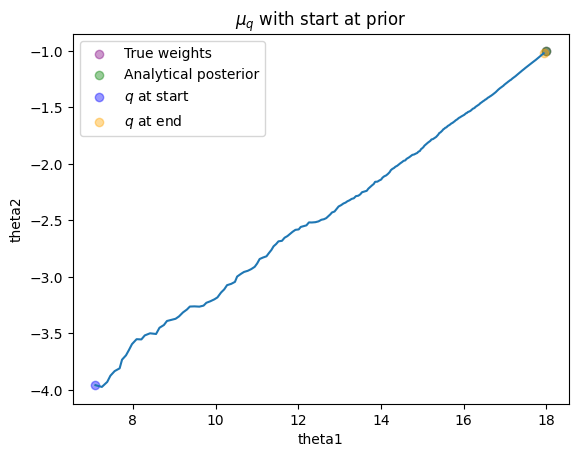
\includegraphics[width=\textwidth]{week3/mu-walk-1.png}
  \end{subfigure}
  \begin{subfigure}{0.4\textwidth}
    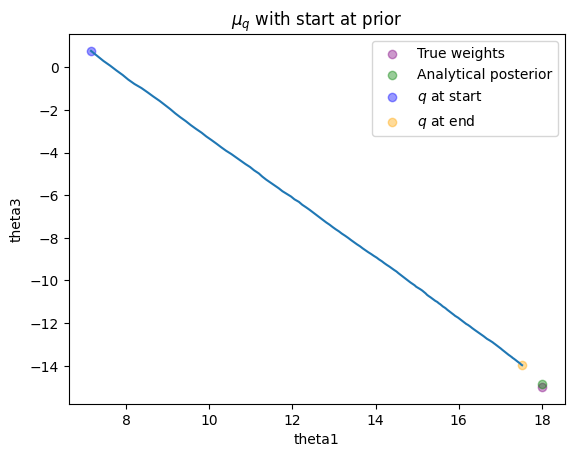
\includegraphics[width=\textwidth]{week3/mu-walk-2.png}
  \end{subfigure}
  \caption{Change in mean of $q$ after 200 iterations of the algorithm with $N$ = 10, $\ell = 100$.}
  \label{fig:mu-walk}
\end{figure}
\begin{figure}[H]
  \centering
  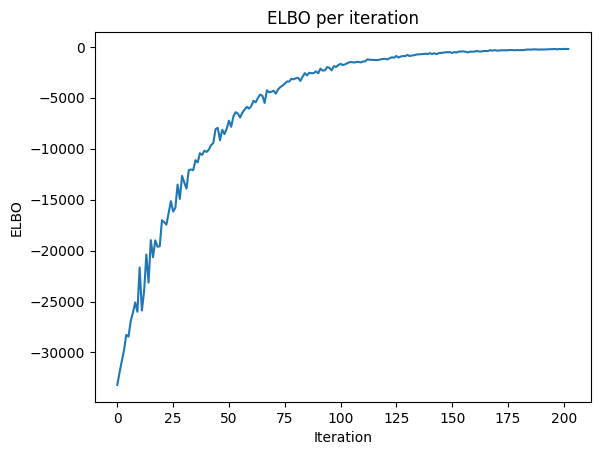
\includegraphics[width=0.5\textwidth]{week3/elbo-per-iter.png}
  \caption{ELBO after each iteration of the algorithm with $N$ = 10, $\ell = 100$.}
  \label{fig:elbo}
\end{figure}
As one can see in Figure \ref{fig:mu-walk}, the mean of $q$ confidently moves towards the analytical posterior (and true weights).
It can also been seen in Figure \ref{fig:elbo} that the ELBO converges after 200 or so iterations, indicating that we have indeed found an optimum.
\subsection{Evaluation}
The algorithm presented here works as expected, and functions as a possible replacement for the analytical posterior.
We've been able to utilize the ELBO as a proxy for the KL-divergence and created a framework that can fitted to many different kind of regression problems, 
as long as one can estimate the log-likelihood and compute the KL-divergence between the variational distribution and the prior.


\end{document}

